%----------------------------------------------------------------------------------------
%    PACKAGES AND THEMES
%----------------------------------------------------------------------------------------

\documentclass[aspectratio=169,xcolor=dvipsnames,t,12pt]{beamer}
\usetheme{SimpleUstbBlue}

\usepackage[UTF8,fontset=windows]{ctex}
\usepackage{amsmath,amssymb,bm,mathtools,tikz}
\usepackage{hyperref,graphicx,booktabs,xcolor,tikz}

\setlength{\emergencystretch}{1em}
\setbeamertemplate{navigation symbols}{}
\setbeamerfont{block title}{size=\normalsize}
\setbeamertemplate{blocks}[rounded][shadow=false]

\definecolor{Teal}{HTML}{087F8C}
\newcommand{\takeaway}[1]{\par\smallskip{\color{Teal}\bfseries#1}\par\smallskip} % \smallskip \medskip \bigskip

\definecolor{Gray}{HTML}{536575}
\newcommand{\source}[1]{%
	\begin{tikzpicture}[remember picture,overlay]
		\node[anchor=south, text width=\textwidth, align=left, font=\tiny\linespread{1.0}\selectfont, yshift=0.3cm] at (current page.south) {\color{Gray}#1};
	\end{tikzpicture}%
}

%----------------------------------------------------------------------------------------
%    TITLE PAGE
%----------------------------------------------------------------------------------------

\title{SimpleUstbBlue Beamer Theme}
\subtitle{Subtitle}

\author{ \\ Lianjun Liu}

\institute
{
    \\ School of Automation and Electrical Engineering \\ University of Science and Technology Beijing
}
\date{\\ \today} % Date, can be changed to a custom date

%----------------------------------------------------------------------------------------
%    PRESENTATION SLIDES
%----------------------------------------------------------------------------------------

\begin{document}

\begin{frame}
    \titlepage
\end{frame}

\begin{frame}{Overview}
    % Throughout your presentation, if you choose to use \section{} and \subsection{} commands, these will automatically be printed on this slide as an overview of your presentation
    \tableofcontents
\end{frame}

%------------------------------------------------
\section{First Section}
%------------------------------------------------

\begin{frame}{Bullet Points}
    \begin{itemize}
        \item Lorem ipsum dolor sit amet, consectetur adipiscing elit
        \item Aliquam blandit faucibus nisi, sit amet dapibus enim tempus eu
        \item Nulla commodo, erat quis gravida posuere, elit lacus lobortis est, quis porttitor odio mauris at libero
        \item Nam cursus est eget velit posuere pellentesque
        \item Vestibulum faucibus velit a augue condimentum quis convallis nulla gravida
    \end{itemize}
\end{frame}

%------------------------------------------------

\begin{frame}{Blocks of Highlighted Text}
    In this slide, some important text will be \alert{highlighted} because it's important. Please, don't abuse it.

    \begin{block}{Block}
        Sample text
    \end{block}

    \begin{alertblock}{Alertblock}
        Sample text in red box
    \end{alertblock}

    \begin{examples}
        Sample text in green box. The title of the block is ``Examples".
    \end{examples}
\end{frame}

%------------------------------------------------

\begin{frame}{Multiple Columns}
    \begin{columns}

        \column{.45\textwidth} % Left column and width
        \textbf{Heading}
        \begin{enumerate}
            \item Statement
            \item Explanation
            \item Example
        \end{enumerate}

        \column{.45\textwidth} % Right column and width
        Lorem ipsum dolor sit amet, consectetur adipiscing elit. Integer lectus nisl, ultricies in feugiat rutrum, porttitor sit amet augue. Aliquam ut tortor mauris. Sed volutpat ante purus, quis accumsan dolor.

    \end{columns}
\end{frame}

%------------------------------------------------
\section{Second Section}
%------------------------------------------------

\begin{frame}{Table}
    \begin{table}
        \begin{tabular}{l l l}
            \toprule
            \textbf{Treatments} & \textbf{Response 1} & \textbf{Response 2} \\
            \midrule
            Treatment 1         & 0.0003262           & 0.562               \\
            Treatment 2         & 0.0015681           & 0.910               \\
            Treatment 3         & 0.0009271           & 0.296               \\
            \bottomrule
        \end{tabular}
        \caption{Table caption}
    \end{table}
\end{frame}

%------------------------------------------------

\begin{frame}{Theorem}
    \begin{theorem}[Mass--energy equivalence]
        $E = mc^2$
    \end{theorem}
    \takeaway{矩阵乘法不满足交换律。}
    \source{这是来源。\\ 这也是来源。}
\end{frame}

%------------------------------------------------

\begin{frame}{Figure}
    Uncomment the code on this slide to include your own image from the same directory as the template .TeX file.
    \begin{figure}
    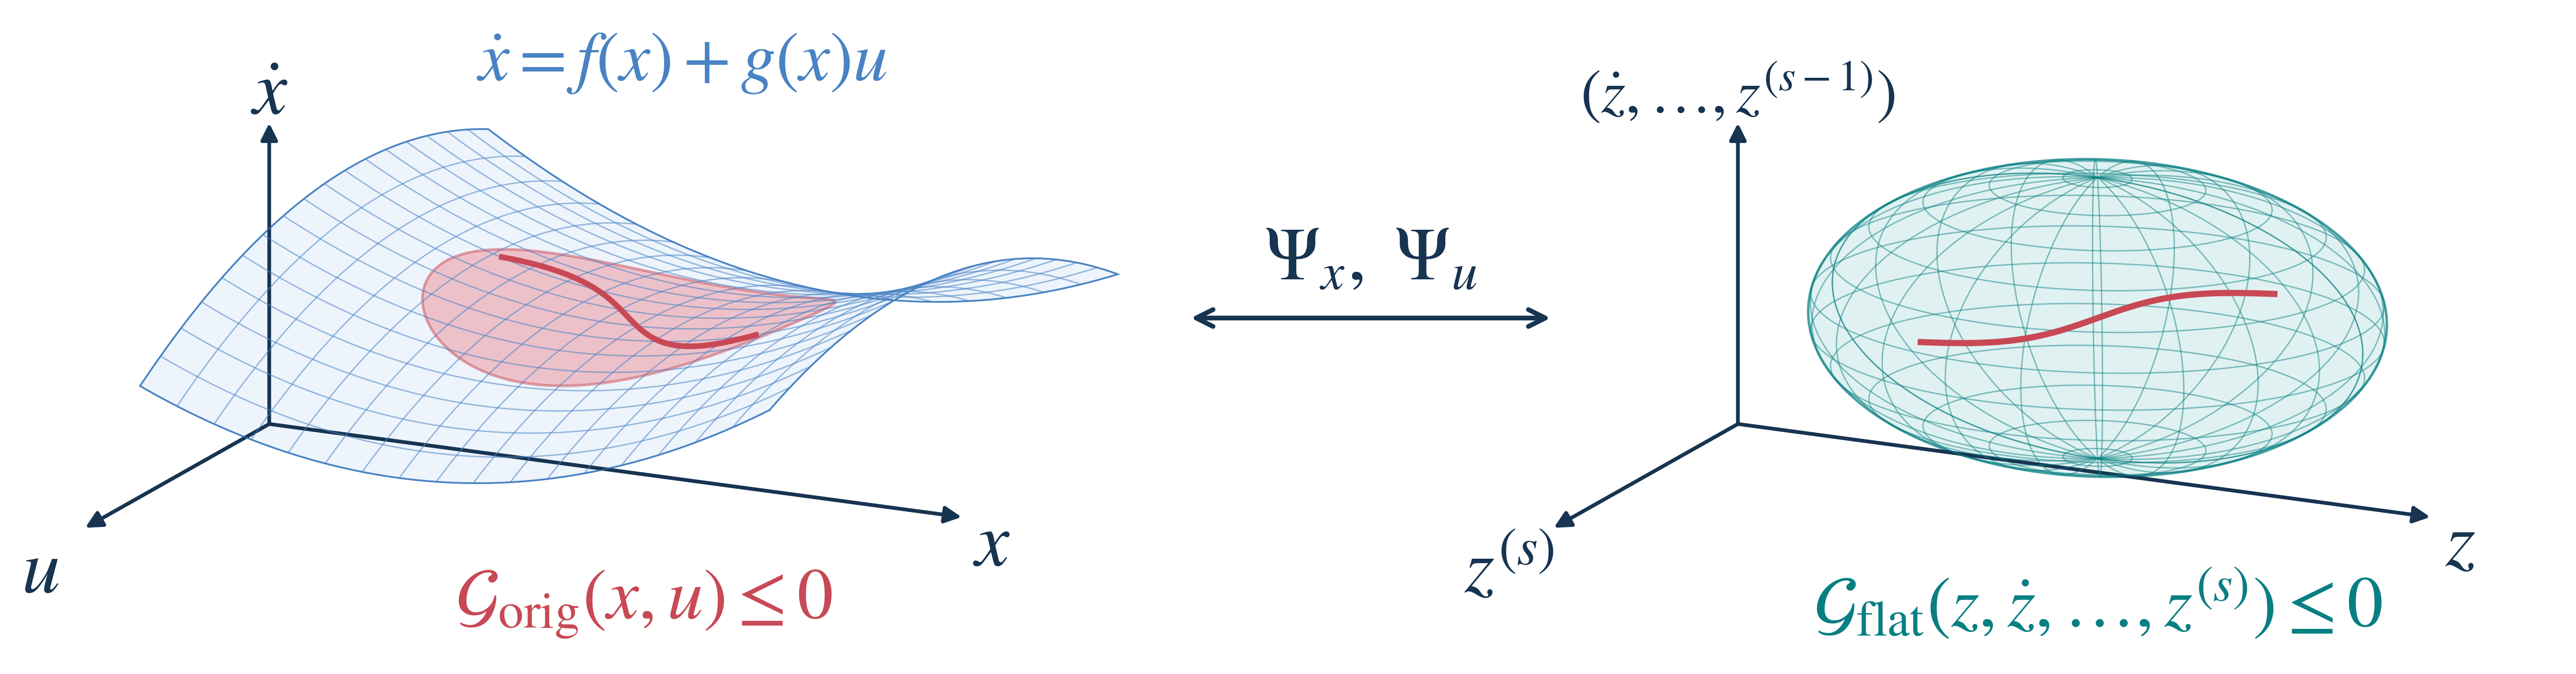
\includegraphics[width=0.8\linewidth]{test}
    \end{figure}
\end{frame}

%------------------------------------------------

\begin{frame}[fragile] % Need to use the fragile option when verbatim is used in the slide
    \frametitle{Citation}
    An example of the \verb|\cite| command to cite within the presentation:\\~

    This statement requires citation \cite{p1}.
\end{frame}

%------------------------------------------------

\begin{frame}{References}
    \footnotesize
    \bibliography{reference.bib}
    \bibliographystyle{apalike}
\end{frame}

%------------------------------------------------

\begin{frame}
	\title{请老师同学批评指正！}
	\subtitle{}
	\titlepage
\end{frame}

%----------------------------------------------------------------------------------------

\end{document}